\chapter{Analisis Data Fisik}

\section{Membuat Data Universal}
Dalam pembuatan data universal ini kita menuliskan semua atribut universal yang dimiliki oleh setiap berkas, sebagai berikut :
\begin{itemize}

	\item Kartu Tanda Penduduk\\
		NIK\\
		Nama\\
		Tempat/Tgl Lahir\\
		Jenis Kelamin\\
		Alamat\\
		RT/RW\\
		Kel/Desa\\
		Kecamatan\\
		Agama\\
		Status Perkawinan\\
		Pekerjaan\\
		Kewarganegaraan\\
		Berlaku Hingga\\
	
		
	\item Formulir Surat Izin Mengemudi\\
		Jenis permohonan\\
		Sim Yang Pernah Dimiliki\\
		Sebutkan Golongan Sim Yang Diminta\\
		Nomor Resi\\
		Nama Depan\\
		Nama Belakang\\


\end{itemize}
Setelah semua data kita analisis maka ini hasil tabel yg sudah kita buat :

\begin{figure}[H]
	\centering
	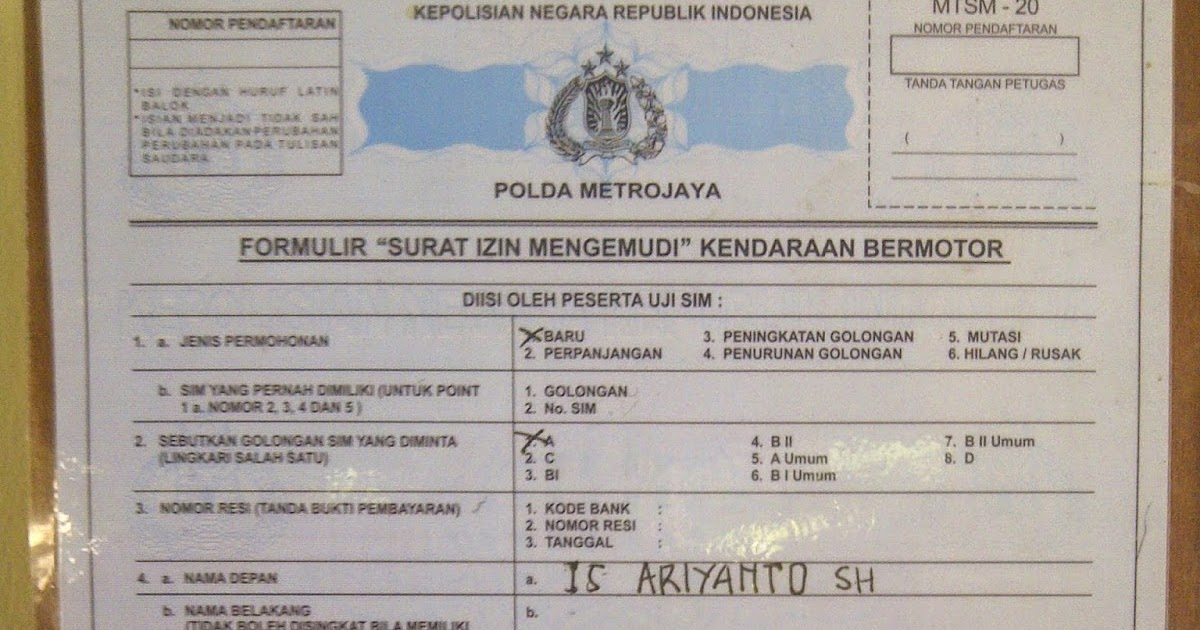
\includegraphics[width=12cm]{figures/syarat.jpg}
	\caption{Tabel Syarat .}	
\end{figure}